% Options for packages loaded elsewhere
\PassOptionsToPackage{unicode}{hyperref}
\PassOptionsToPackage{hyphens}{url}
\PassOptionsToPackage{dvipsnames,svgnames,x11names}{xcolor}
%
\documentclass[
  letterpaper,
  DIV=11,
  numbers=noendperiod]{scrartcl}

\usepackage{amsmath,amssymb}
\usepackage{iftex}
\ifPDFTeX
  \usepackage[T1]{fontenc}
  \usepackage[utf8]{inputenc}
  \usepackage{textcomp} % provide euro and other symbols
\else % if luatex or xetex
  \usepackage{unicode-math}
  \defaultfontfeatures{Scale=MatchLowercase}
  \defaultfontfeatures[\rmfamily]{Ligatures=TeX,Scale=1}
\fi
\usepackage{lmodern}
\ifPDFTeX\else  
    % xetex/luatex font selection
\fi
% Use upquote if available, for straight quotes in verbatim environments
\IfFileExists{upquote.sty}{\usepackage{upquote}}{}
\IfFileExists{microtype.sty}{% use microtype if available
  \usepackage[]{microtype}
  \UseMicrotypeSet[protrusion]{basicmath} % disable protrusion for tt fonts
}{}
\makeatletter
\@ifundefined{KOMAClassName}{% if non-KOMA class
  \IfFileExists{parskip.sty}{%
    \usepackage{parskip}
  }{% else
    \setlength{\parindent}{0pt}
    \setlength{\parskip}{6pt plus 2pt minus 1pt}}
}{% if KOMA class
  \KOMAoptions{parskip=half}}
\makeatother
\usepackage{xcolor}
\setlength{\emergencystretch}{3em} % prevent overfull lines
\setcounter{secnumdepth}{-\maxdimen} % remove section numbering
% Make \paragraph and \subparagraph free-standing
\makeatletter
\ifx\paragraph\undefined\else
  \let\oldparagraph\paragraph
  \renewcommand{\paragraph}{
    \@ifstar
      \xxxParagraphStar
      \xxxParagraphNoStar
  }
  \newcommand{\xxxParagraphStar}[1]{\oldparagraph*{#1}\mbox{}}
  \newcommand{\xxxParagraphNoStar}[1]{\oldparagraph{#1}\mbox{}}
\fi
\ifx\subparagraph\undefined\else
  \let\oldsubparagraph\subparagraph
  \renewcommand{\subparagraph}{
    \@ifstar
      \xxxSubParagraphStar
      \xxxSubParagraphNoStar
  }
  \newcommand{\xxxSubParagraphStar}[1]{\oldsubparagraph*{#1}\mbox{}}
  \newcommand{\xxxSubParagraphNoStar}[1]{\oldsubparagraph{#1}\mbox{}}
\fi
\makeatother

\usepackage{color}
\usepackage{fancyvrb}
\newcommand{\VerbBar}{|}
\newcommand{\VERB}{\Verb[commandchars=\\\{\}]}
\DefineVerbatimEnvironment{Highlighting}{Verbatim}{commandchars=\\\{\}}
% Add ',fontsize=\small' for more characters per line
\usepackage{framed}
\definecolor{shadecolor}{RGB}{241,243,245}
\newenvironment{Shaded}{\begin{snugshade}}{\end{snugshade}}
\newcommand{\AlertTok}[1]{\textcolor[rgb]{0.68,0.00,0.00}{#1}}
\newcommand{\AnnotationTok}[1]{\textcolor[rgb]{0.37,0.37,0.37}{#1}}
\newcommand{\AttributeTok}[1]{\textcolor[rgb]{0.40,0.45,0.13}{#1}}
\newcommand{\BaseNTok}[1]{\textcolor[rgb]{0.68,0.00,0.00}{#1}}
\newcommand{\BuiltInTok}[1]{\textcolor[rgb]{0.00,0.23,0.31}{#1}}
\newcommand{\CharTok}[1]{\textcolor[rgb]{0.13,0.47,0.30}{#1}}
\newcommand{\CommentTok}[1]{\textcolor[rgb]{0.37,0.37,0.37}{#1}}
\newcommand{\CommentVarTok}[1]{\textcolor[rgb]{0.37,0.37,0.37}{\textit{#1}}}
\newcommand{\ConstantTok}[1]{\textcolor[rgb]{0.56,0.35,0.01}{#1}}
\newcommand{\ControlFlowTok}[1]{\textcolor[rgb]{0.00,0.23,0.31}{\textbf{#1}}}
\newcommand{\DataTypeTok}[1]{\textcolor[rgb]{0.68,0.00,0.00}{#1}}
\newcommand{\DecValTok}[1]{\textcolor[rgb]{0.68,0.00,0.00}{#1}}
\newcommand{\DocumentationTok}[1]{\textcolor[rgb]{0.37,0.37,0.37}{\textit{#1}}}
\newcommand{\ErrorTok}[1]{\textcolor[rgb]{0.68,0.00,0.00}{#1}}
\newcommand{\ExtensionTok}[1]{\textcolor[rgb]{0.00,0.23,0.31}{#1}}
\newcommand{\FloatTok}[1]{\textcolor[rgb]{0.68,0.00,0.00}{#1}}
\newcommand{\FunctionTok}[1]{\textcolor[rgb]{0.28,0.35,0.67}{#1}}
\newcommand{\ImportTok}[1]{\textcolor[rgb]{0.00,0.46,0.62}{#1}}
\newcommand{\InformationTok}[1]{\textcolor[rgb]{0.37,0.37,0.37}{#1}}
\newcommand{\KeywordTok}[1]{\textcolor[rgb]{0.00,0.23,0.31}{\textbf{#1}}}
\newcommand{\NormalTok}[1]{\textcolor[rgb]{0.00,0.23,0.31}{#1}}
\newcommand{\OperatorTok}[1]{\textcolor[rgb]{0.37,0.37,0.37}{#1}}
\newcommand{\OtherTok}[1]{\textcolor[rgb]{0.00,0.23,0.31}{#1}}
\newcommand{\PreprocessorTok}[1]{\textcolor[rgb]{0.68,0.00,0.00}{#1}}
\newcommand{\RegionMarkerTok}[1]{\textcolor[rgb]{0.00,0.23,0.31}{#1}}
\newcommand{\SpecialCharTok}[1]{\textcolor[rgb]{0.37,0.37,0.37}{#1}}
\newcommand{\SpecialStringTok}[1]{\textcolor[rgb]{0.13,0.47,0.30}{#1}}
\newcommand{\StringTok}[1]{\textcolor[rgb]{0.13,0.47,0.30}{#1}}
\newcommand{\VariableTok}[1]{\textcolor[rgb]{0.07,0.07,0.07}{#1}}
\newcommand{\VerbatimStringTok}[1]{\textcolor[rgb]{0.13,0.47,0.30}{#1}}
\newcommand{\WarningTok}[1]{\textcolor[rgb]{0.37,0.37,0.37}{\textit{#1}}}

\providecommand{\tightlist}{%
  \setlength{\itemsep}{0pt}\setlength{\parskip}{0pt}}\usepackage{longtable,booktabs,array}
\usepackage{calc} % for calculating minipage widths
% Correct order of tables after \paragraph or \subparagraph
\usepackage{etoolbox}
\makeatletter
\patchcmd\longtable{\par}{\if@noskipsec\mbox{}\fi\par}{}{}
\makeatother
% Allow footnotes in longtable head/foot
\IfFileExists{footnotehyper.sty}{\usepackage{footnotehyper}}{\usepackage{footnote}}
\makesavenoteenv{longtable}
\usepackage{graphicx}
\makeatletter
\newsavebox\pandoc@box
\newcommand*\pandocbounded[1]{% scales image to fit in text height/width
  \sbox\pandoc@box{#1}%
  \Gscale@div\@tempa{\textheight}{\dimexpr\ht\pandoc@box+\dp\pandoc@box\relax}%
  \Gscale@div\@tempb{\linewidth}{\wd\pandoc@box}%
  \ifdim\@tempb\p@<\@tempa\p@\let\@tempa\@tempb\fi% select the smaller of both
  \ifdim\@tempa\p@<\p@\scalebox{\@tempa}{\usebox\pandoc@box}%
  \else\usebox{\pandoc@box}%
  \fi%
}
% Set default figure placement to htbp
\def\fps@figure{htbp}
\makeatother

\KOMAoption{captions}{tableheading}
\makeatletter
\@ifpackageloaded{caption}{}{\usepackage{caption}}
\AtBeginDocument{%
\ifdefined\contentsname
  \renewcommand*\contentsname{Table of contents}
\else
  \newcommand\contentsname{Table of contents}
\fi
\ifdefined\listfigurename
  \renewcommand*\listfigurename{List of Figures}
\else
  \newcommand\listfigurename{List of Figures}
\fi
\ifdefined\listtablename
  \renewcommand*\listtablename{List of Tables}
\else
  \newcommand\listtablename{List of Tables}
\fi
\ifdefined\figurename
  \renewcommand*\figurename{Figure}
\else
  \newcommand\figurename{Figure}
\fi
\ifdefined\tablename
  \renewcommand*\tablename{Table}
\else
  \newcommand\tablename{Table}
\fi
}
\@ifpackageloaded{float}{}{\usepackage{float}}
\floatstyle{ruled}
\@ifundefined{c@chapter}{\newfloat{codelisting}{h}{lop}}{\newfloat{codelisting}{h}{lop}[chapter]}
\floatname{codelisting}{Listing}
\newcommand*\listoflistings{\listof{codelisting}{List of Listings}}
\makeatother
\makeatletter
\makeatother
\makeatletter
\@ifpackageloaded{caption}{}{\usepackage{caption}}
\@ifpackageloaded{subcaption}{}{\usepackage{subcaption}}
\makeatother

\usepackage{bookmark}

\IfFileExists{xurl.sty}{\usepackage{xurl}}{} % add URL line breaks if available
\urlstyle{same} % disable monospaced font for URLs
\hypersetup{
  pdftitle={Relatorio\_Maria\_Carolina},
  colorlinks=true,
  linkcolor={blue},
  filecolor={Maroon},
  citecolor={Blue},
  urlcolor={Blue},
  pdfcreator={LaTeX via pandoc}}


\title{Relatorio\_Maria\_Carolina}
\author{}
\date{}

\begin{document}
\maketitle


\subsection{Análise de Risco e Retorno
:}\label{anuxe1lise-de-risco-e-retorno}

Nesta etapa, foi realizada uma análise dos \textbf{preços de fechamento
dos ativos} no período de \textbf{01/04/2025 a 27/06/2025}, com o
objetivo de compreender a dinâmica histórica e apoiar decisões futuras
de investimento. A partir da estratégia \textbf{buy and hold} e do
referencial \textbf{teórico de benchmark}, foram identificados:

\begin{itemize}
\item
  O \textbf{preço inicial} e \textbf{preço final} da série
\item
  O \textbf{menor} e o \textbf{maior valor} registrado no período,
\item
  E a \textbf{variação percentual teórica} entre esses pontos,
  representando o potencial de crescimento ou retração do ativo.
\item
  Esses indicadores permitem observar a trajetória dos ativos e avaliar
  sua performance em termos de risco e retorno. O intuito é entender o
  comportamento passado para \textbf{operar de forma mais estratégica no
  futuro}.
\end{itemize}

Os dados utilizados foram carregados via script, considerando todos os
ativos da carteira em análise.

\begin{Shaded}
\begin{Highlighting}[]
\FunctionTok{library}\NormalTok{(tseries)}
\end{Highlighting}
\end{Shaded}

\begin{verbatim}
Registered S3 method overwritten by 'quantmod':
  method            from
  as.zoo.data.frame zoo 
\end{verbatim}

\begin{Shaded}
\begin{Highlighting}[]
\CommentTok{\# Datas de início e fim}
\NormalTok{dataini }\OtherTok{\textless{}{-}} \FunctionTok{as.Date}\NormalTok{(}\StringTok{"2025{-}04{-}01"}\NormalTok{)}
\NormalTok{datafim }\OtherTok{\textless{}{-}} \FunctionTok{as.Date}\NormalTok{(}\StringTok{"2025{-}06{-}28"}\NormalTok{)}

\CommentTok{\# Baixando os dados dos 5 ativos}
\NormalTok{lwsa3  }\OtherTok{\textless{}{-}} \FunctionTok{get.hist.quote}\NormalTok{(}\StringTok{"lwsa3.sa"}\NormalTok{,  }\AttributeTok{quote =} \StringTok{"Close"}\NormalTok{, }\AttributeTok{start =}\NormalTok{ dataini, }\AttributeTok{end =}\NormalTok{ datafim)}
\end{Highlighting}
\end{Shaded}

\begin{verbatim}
time series ends   2025-06-27
\end{verbatim}

\begin{Shaded}
\begin{Highlighting}[]
\NormalTok{elet6 }\OtherTok{\textless{}{-}} \FunctionTok{get.hist.quote}\NormalTok{(}\StringTok{"elet6.sa"}\NormalTok{,  }\AttributeTok{quote =} \StringTok{"Close"}\NormalTok{, }\AttributeTok{start =}\NormalTok{ dataini, }\AttributeTok{end =}\NormalTok{ datafim)}
\end{Highlighting}
\end{Shaded}

\begin{verbatim}
time series ends   2025-06-27
\end{verbatim}

\begin{Shaded}
\begin{Highlighting}[]
\NormalTok{itsa4  }\OtherTok{\textless{}{-}} \FunctionTok{get.hist.quote}\NormalTok{(}\StringTok{"itsa4.sa"}\NormalTok{,  }\AttributeTok{quote =} \StringTok{"Close"}\NormalTok{, }\AttributeTok{start =}\NormalTok{ dataini, }\AttributeTok{end =}\NormalTok{ datafim)}
\end{Highlighting}
\end{Shaded}

\begin{verbatim}
time series ends   2025-06-27
\end{verbatim}

\begin{Shaded}
\begin{Highlighting}[]
\NormalTok{rent3  }\OtherTok{\textless{}{-}} \FunctionTok{get.hist.quote}\NormalTok{(}\StringTok{"rent3.sa"}\NormalTok{,  }\AttributeTok{quote =} \StringTok{"Close"}\NormalTok{, }\AttributeTok{start =}\NormalTok{ dataini, }\AttributeTok{end =}\NormalTok{ datafim)}
\end{Highlighting}
\end{Shaded}

\begin{verbatim}
time series ends   2025-06-27
\end{verbatim}

\begin{Shaded}
\begin{Highlighting}[]
\NormalTok{brfs3  }\OtherTok{\textless{}{-}} \FunctionTok{get.hist.quote}\NormalTok{(}\StringTok{"brfs3.sa"}\NormalTok{,  }\AttributeTok{quote =} \StringTok{"Close"}\NormalTok{, }\AttributeTok{start =}\NormalTok{ dataini, }\AttributeTok{end =}\NormalTok{ datafim)}
\end{Highlighting}
\end{Shaded}

\begin{verbatim}
time series ends   2025-06-27
\end{verbatim}

\begin{Shaded}
\begin{Highlighting}[]
\CommentTok{\# Removendo valores ausentes}
\NormalTok{lwsa3 }\OtherTok{\textless{}{-}} \FunctionTok{na.omit}\NormalTok{(lwsa3)}
\NormalTok{elet6 }\OtherTok{\textless{}{-}} \FunctionTok{na.omit}\NormalTok{(elet6)}
\NormalTok{itsa4 }\OtherTok{\textless{}{-}} \FunctionTok{na.omit}\NormalTok{(itsa4)}
\NormalTok{rent3 }\OtherTok{\textless{}{-}} \FunctionTok{na.omit}\NormalTok{(rent3)}
\NormalTok{brfs3 }\OtherTok{\textless{}{-}} \FunctionTok{na.omit}\NormalTok{(brfs3)}

\CommentTok{\# Verificando quantidade de observações e visualizando os dados}
\FunctionTok{length}\NormalTok{(lwsa3); }\FunctionTok{plot}\NormalTok{(lwsa3, }\AttributeTok{main =} \StringTok{"Análise da teoria Dow {-} LWSA3"}\NormalTok{)}
\end{Highlighting}
\end{Shaded}

\begin{verbatim}
[1] 60
\end{verbatim}

\pandocbounded{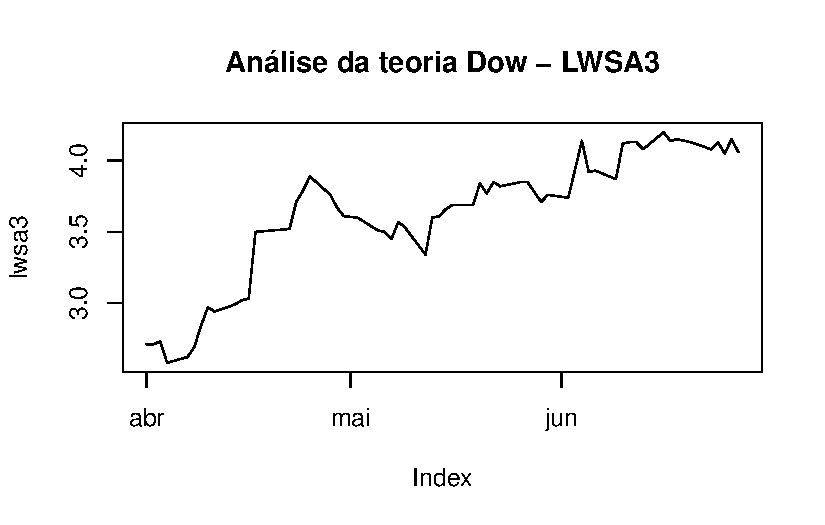
\includegraphics[keepaspectratio]{Relatorio_Maria_Carolina_files/figure-pdf/unnamed-chunk-1-1.pdf}}

\begin{Shaded}
\begin{Highlighting}[]
\FunctionTok{length}\NormalTok{(elet6); }\FunctionTok{plot}\NormalTok{(elet6, }\AttributeTok{main =} \StringTok{"Análise da teoria Dow{-} ELET6"}\NormalTok{)}
\end{Highlighting}
\end{Shaded}

\begin{verbatim}
[1] 60
\end{verbatim}

\pandocbounded{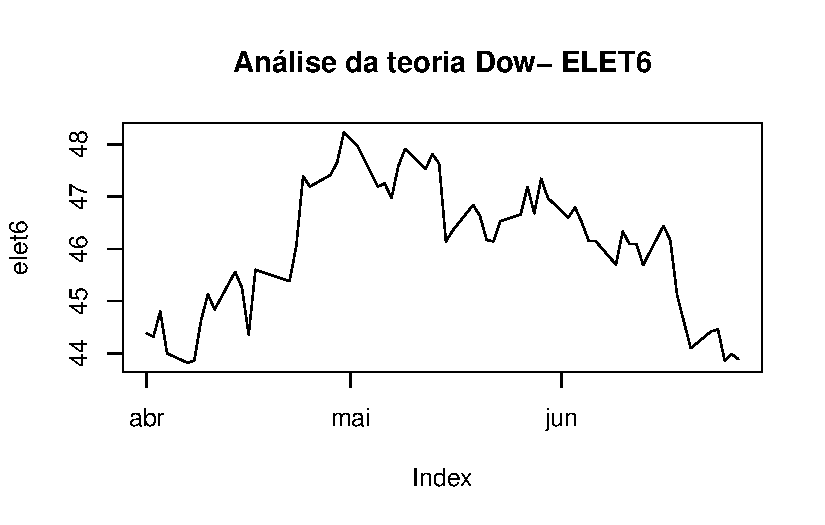
\includegraphics[keepaspectratio]{Relatorio_Maria_Carolina_files/figure-pdf/unnamed-chunk-1-2.pdf}}

\begin{Shaded}
\begin{Highlighting}[]
\FunctionTok{length}\NormalTok{(itsa4); }\FunctionTok{plot}\NormalTok{(itsa4, }\AttributeTok{main =} \StringTok{"Análise da teoria Dow {-} ITSA4"}\NormalTok{)}
\end{Highlighting}
\end{Shaded}

\begin{verbatim}
[1] 60
\end{verbatim}

\pandocbounded{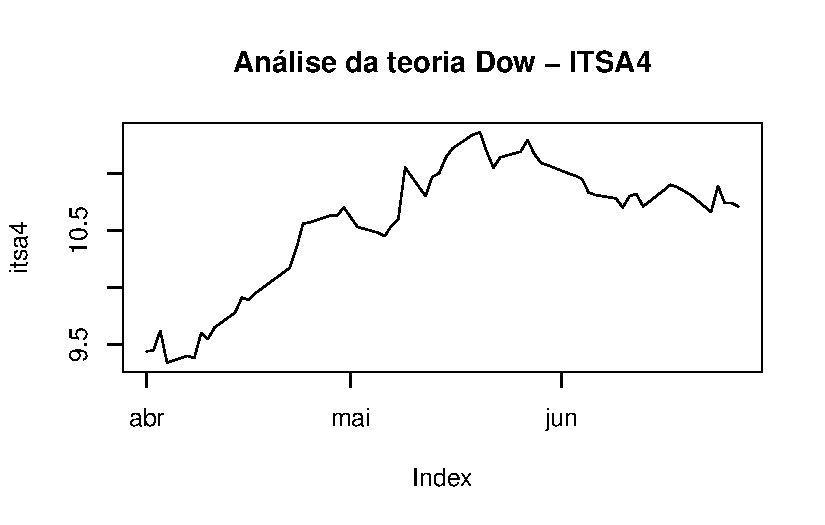
\includegraphics[keepaspectratio]{Relatorio_Maria_Carolina_files/figure-pdf/unnamed-chunk-1-3.pdf}}

\begin{Shaded}
\begin{Highlighting}[]
\FunctionTok{length}\NormalTok{(rent3); }\FunctionTok{plot}\NormalTok{(rent3, }\AttributeTok{main =} \StringTok{"Análise da teoria Dow {-} rent3"}\NormalTok{)}
\end{Highlighting}
\end{Shaded}

\begin{verbatim}
[1] 60
\end{verbatim}

\pandocbounded{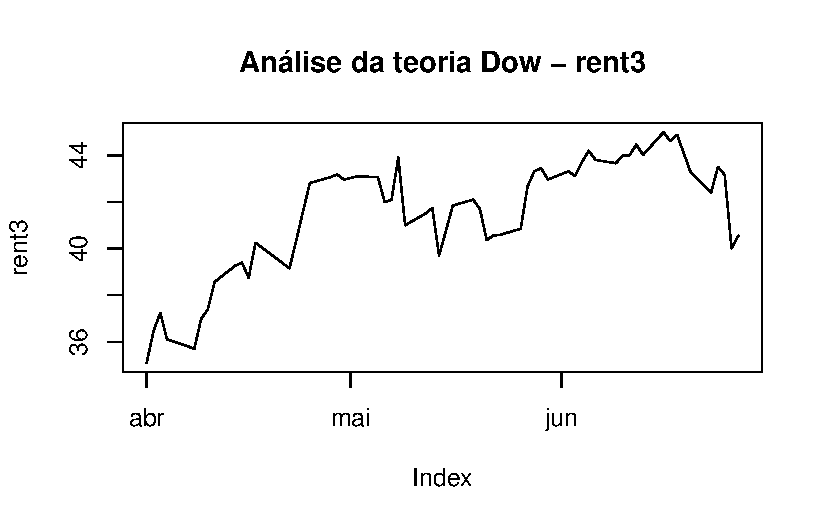
\includegraphics[keepaspectratio]{Relatorio_Maria_Carolina_files/figure-pdf/unnamed-chunk-1-4.pdf}}

\begin{Shaded}
\begin{Highlighting}[]
\FunctionTok{length}\NormalTok{(brfs3); }\FunctionTok{plot}\NormalTok{(brfs3, }\AttributeTok{main =} \StringTok{"Análise da teoria Dow {-} BRFS3"}\NormalTok{)}
\end{Highlighting}
\end{Shaded}

\begin{verbatim}
[1] 60
\end{verbatim}

\pandocbounded{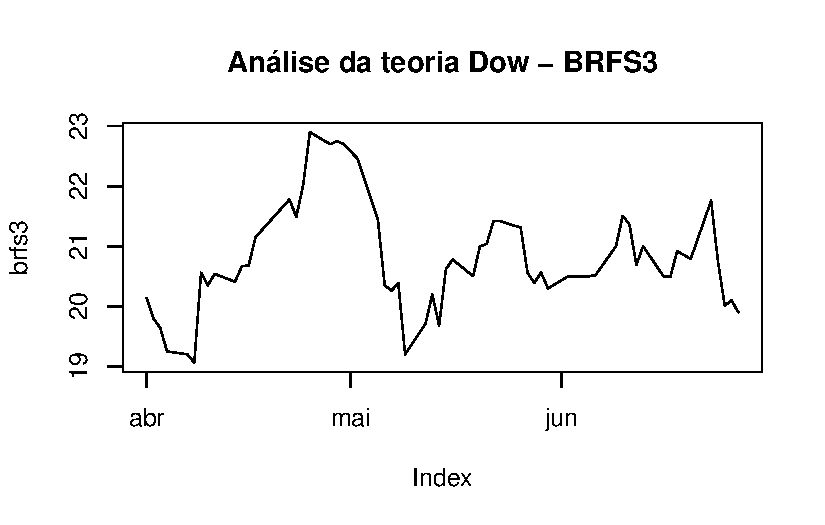
\includegraphics[keepaspectratio]{Relatorio_Maria_Carolina_files/figure-pdf/unnamed-chunk-1-5.pdf}}

\paragraph{Gráficos da análise de risco e
retorno:}\label{gruxe1ficos-da-anuxe1lise-de-risco-e-retorno}

\begin{itemize}
\tightlist
\item
  A análise do ativo \textbf{ITSA4}, representada no gráfico, mostra uma
  valorização de \textbf{3,17 unidades ou 38,67\%} ao longo de
  \textbf{78 candles (114 dias)}, com um volume negociado de
  \textbf{2,56 bilhões} no período. Esse movimento indica uma forte
  tendência de alta, com topos e fundos ascendentes, especialmente no
  início da série. A valorização expressiva sugere \textbf{potencial de
  ganho}, principalmente para estratégias de médio prazo. Para o
  investidor avesso ao risco, essa trajetória pode ser interpretada como
  \textbf{positiva}, desde que acompanhada de fundamentos sólidos, pois
  o padrão gráfico mostra \textbf{uma aceleração consistente} antes de
  entrar em lateralização, o que reduz a volatilidade e favorece a
  previsibilidade.
\end{itemize}

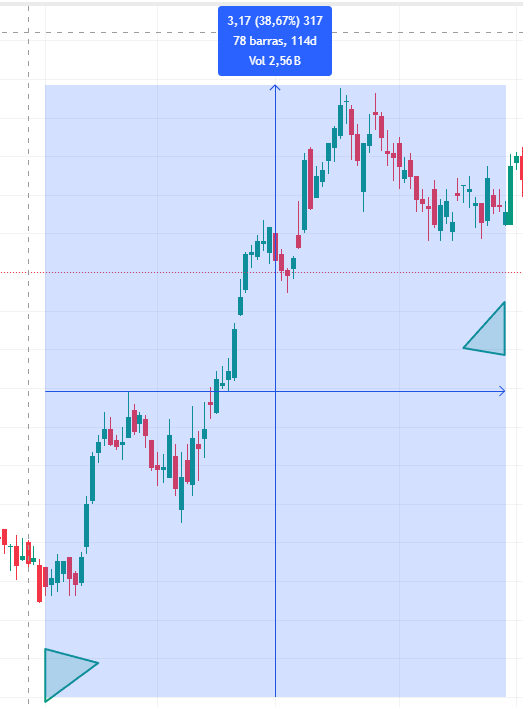
\includegraphics[width=3.47917in,height=\textheight,keepaspectratio]{images/BHA_ITSA4-01.PNG}

\begin{itemize}
\tightlist
\item
  \textbf{teórico de benchmark}
\end{itemize}

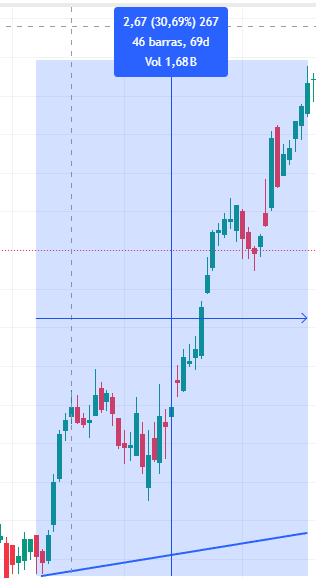
\includegraphics[width=3.44792in,height=\textheight,keepaspectratio]{images/clipboard-3626293039.png}

\begin{itemize}
\item
  No caso do ativo \textbf{BRFS3}, o gráfico indica uma valorização de
  \textbf{6,26 unidades ou 36,63\%} em \textbf{77 candles (113 dias)},
  com volume total de \textbf{714,11 milhões} negociados. O movimento é
  caracterizado por uma \textbf{fase inicial de acumulação}, seguida por
  uma forte alta e posterior estabilização lateral. Esse comportamento
  reflete uma \textbf{tendência de crescimento seguida de consolidação},
  o que pode representar uma \textbf{oportunidade para perfis
  moderados}. No entanto, para investidores avessos ao risco, a
  oscilação após o pico exige cautela, pois a instabilidade na segunda
  metade do período pode indicar \textbf{perda de força compradora} ou
  transição de tendência.

  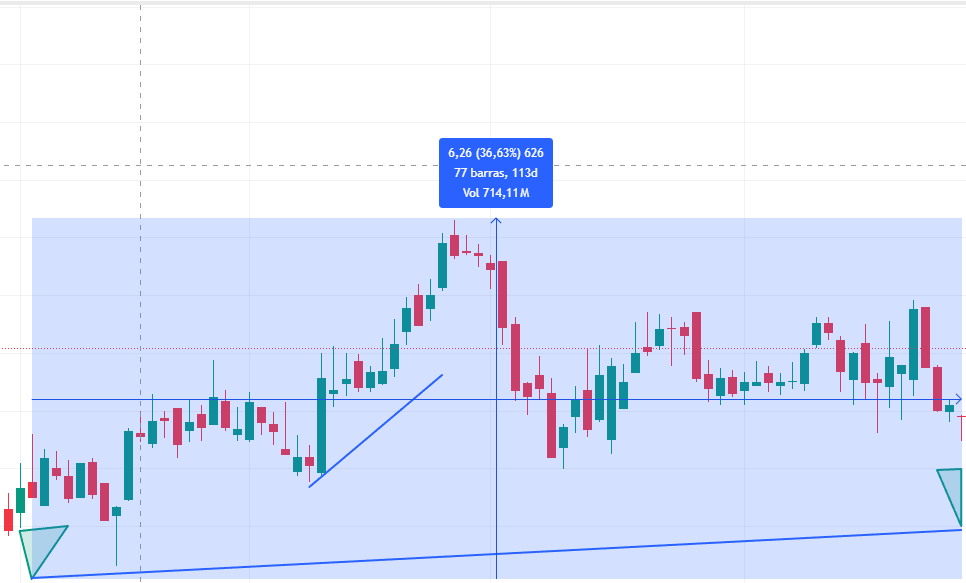
\includegraphics[width=4.55208in,height=\textheight,keepaspectratio]{images/BAH_BRFS3.PNG}
\item
  \textbf{teórico de benchmark}
\end{itemize}

\begin{verbatim}
![](images/TEORICA_BRFS3.PNG){width="498"}
\end{verbatim}

\begin{itemize}
\item
  No caso do ativo ELET6

  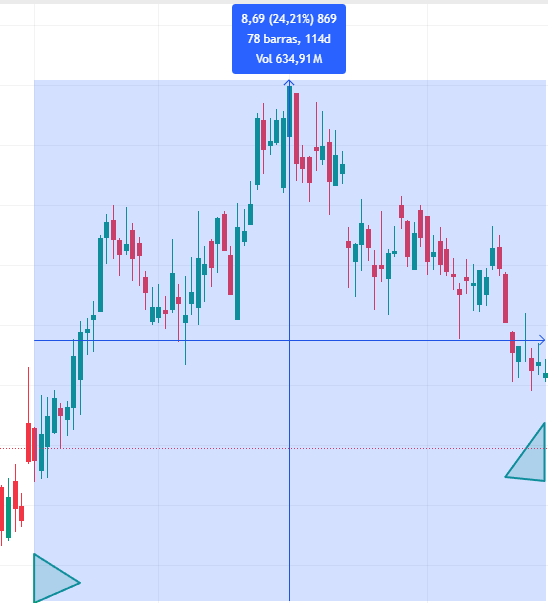
\includegraphics[width=3.98958in,height=\textheight,keepaspectratio]{images/BHA_ELE6-01.PNG}
\item
  \textbf{teórico de benchmark}
\end{itemize}

\begin{verbatim}
![](images/TEORICA_elet6.PNG){width="386"}
\end{verbatim}

\begin{itemize}
\item
  No caso do ativo RENT3

  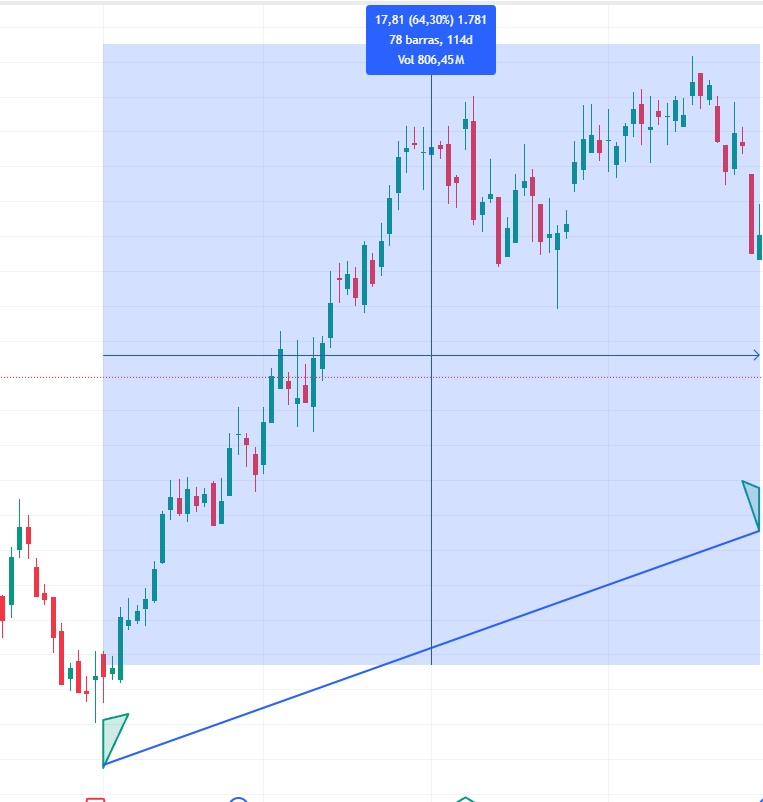
\includegraphics[width=3.42708in,height=\textheight,keepaspectratio]{images/BAH_RENT3.PNG}
\item
  \textbf{teórico de benchmark}
\end{itemize}

\begin{verbatim}
![](images/TEORICA_RENT3.PNG){width="337"}
\end{verbatim}

\begin{itemize}
\item
  No caso do ativo LWSA3
\item
  \textbf{teórico de benchmark}
\end{itemize}

\begin{verbatim}
![](images/TEORICA_LWSA3.PNG){width="379"}

## Análise Aplicando a Teoria de Dow 

Nessa parte busquei também as tendência(sucetiveis repetições de altas e baixas nos preços dos ativos) e ao ligá-los verificar o ângulo da inclinação que exprime a intensidade emocional no mercado nesse dia.

No ativo RENT3 podemos verificar que , ao unimos as linhas de tendências temos muitos momentos de acumulação e alta sensível (representados nas linhas de cor azul) representa um ótimo momento para faturar e nas de baixa verificamos os pontos de distribuição e baixa sensível que nos mostra o sinvestidores vão se desfazendo de suas posições tendencia primaria
\end{verbatim}

\begin{itemize}
\item
  Análise do ativo BRFS3:

  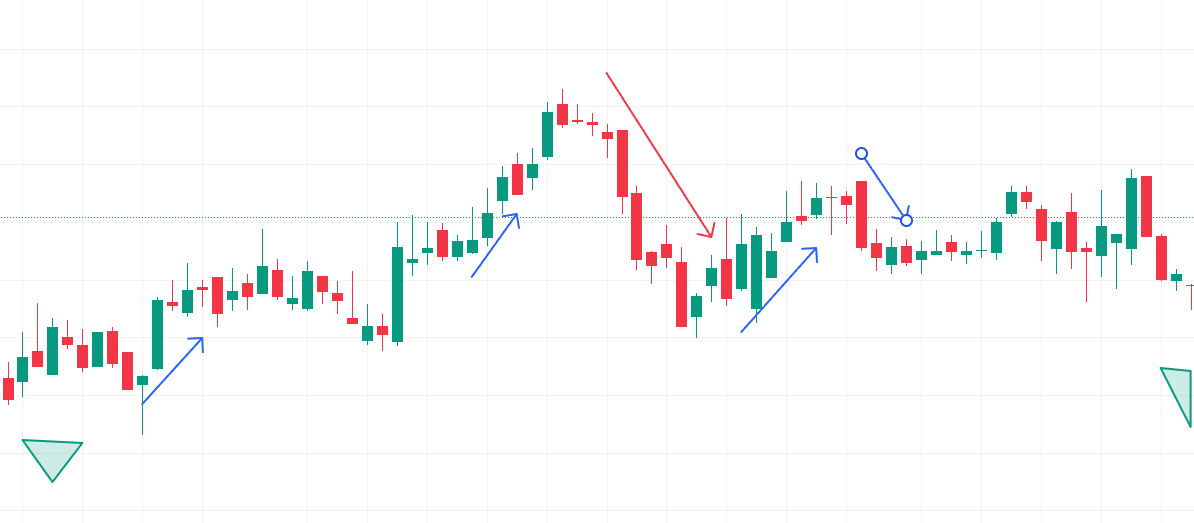
\includegraphics[width=6.35417in,height=\textheight,keepaspectratio]{images/dow2_brfs3.PNG}
\item
  Análise do ativo ELET6 :

  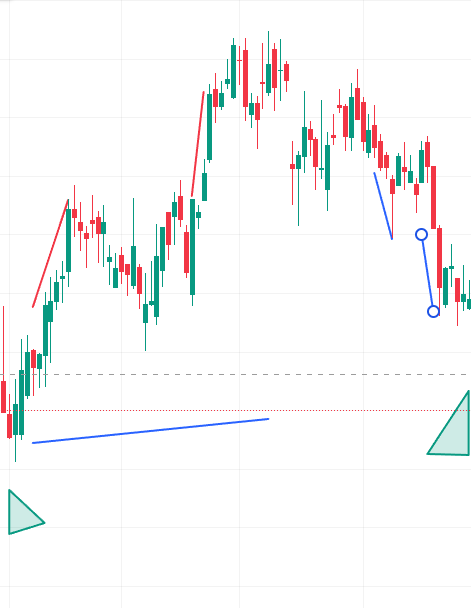
\includegraphics[width=4.5in,height=\textheight,keepaspectratio]{images/dow2_elet6.PNG}
\item
  Análise do ativo ITSA6:

  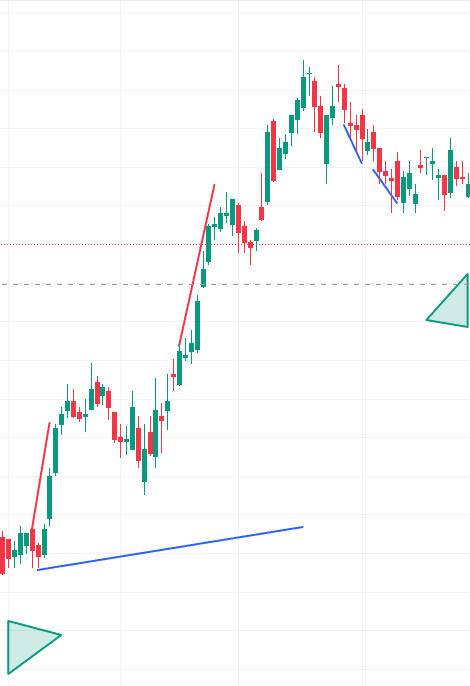
\includegraphics[width=4.46875in,height=\textheight,keepaspectratio]{images/dow2_ITSA4.PNG}
\item
  Análise do ativo RENT3:

  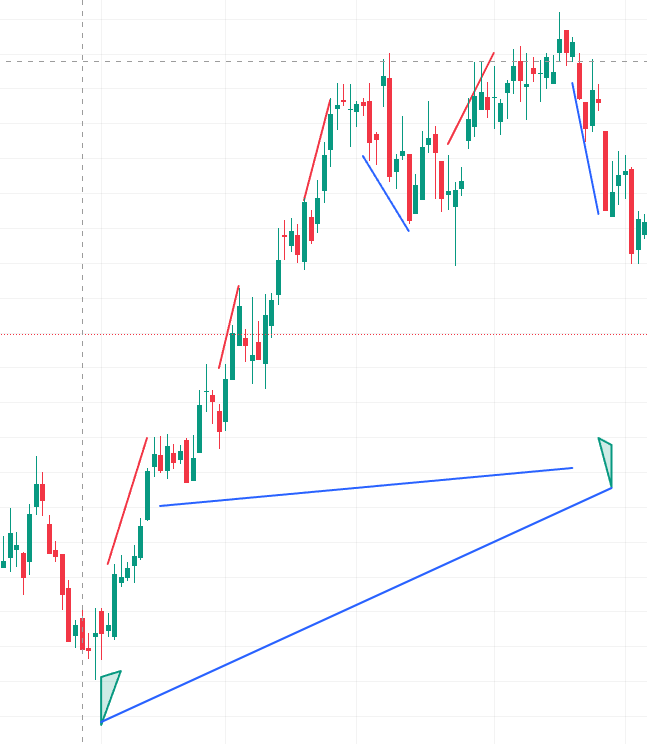
\includegraphics[width=4.10417in,height=\textheight,keepaspectratio]{images/dow2_RENT3.PNG}
\item
  Análise do ativo LWSA3:

  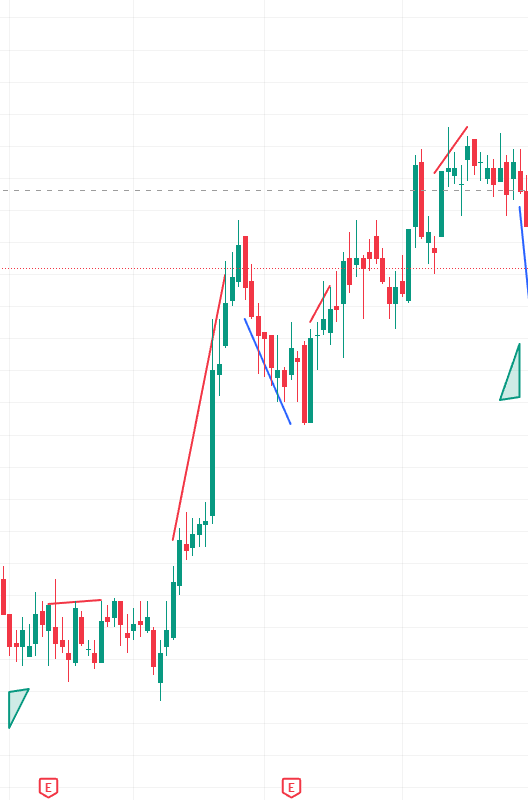
\includegraphics[width=3.85417in,height=\textheight,keepaspectratio]{images/dow2_LSWA.PNG}
\end{itemize}

\subsection{Indicadores Médias Moveis
e}\label{indicadores-muxe9dias-moveis-e}




\end{document}
